% =============================================================
% Pulled by Pixels: Cross-Modal Numerical Anchoring in VLMs
% EMNLP submission outline -- full English translation of emnlp_outline_ko.md
% Compiles with standard pdfLaTeX (ACL/EMNLP default).
%
% Compile: pdflatex main.tex && bibtex main && pdflatex main.tex && pdflatex main.tex
% =============================================================

\documentclass[11pt]{article}

% Change "review" to "final" for the camera-ready, "preprint" for non-anonymous with page numbers.
\usepackage[review]{acl}

% NOTE: acl.sty already loads xcolor, geometry, caption, natbib, hyperref, lineno (review).
% Do NOT add \usepackage{hyperref} or \usepackage{url} -- they will clash.

\usepackage[T1]{fontenc}
\usepackage[utf8]{inputenc}
\usepackage{microtype}
\usepackage{graphicx}
\usepackage[export]{adjustbox}    % for valign=c on includegraphics inside tabular
\usepackage{booktabs}
\usepackage{multirow}
\usepackage{array}
\usepackage{amsmath}
\usepackage{amssymb}

% Convenience macro for outline placeholders that still need authoring.
\newcommand{\todoNote}[1]{\textit{\textcolor[rgb]{0.45,0.45,0.45}{[#1]}}}

\title{Pulled by Pixels: Cross-Modal Numerical Anchoring in VLMs}

\author{Anonymous Submission \\
  \texttt{anonymous@anonymous} \\}

\begin{document}
\maketitle

% =============================================================
\begin{abstract}
\todoNote{Target length $\sim$180 words. Condense the five beats below into a single paragraph.}
\textbf{Problem.}
When a vision--language model (VLM) is shown a question together with an irrelevant image that contains a number, is the model's numeric answer pulled toward that number---a phenomenon we call \textit{cross-modal numerical anchoring}?
\textbf{Finding 1 (phenomenon).}
Across six open-weight VLMs and five datasets, roughly 10--40\,\% of responses are \textit{gradually} pulled toward the anchor digit, and a subset (1.7--15.7\,\%) is even copied verbatim. The magnitude of the pull is larger when the model's confidence in its base answer is lower.
\textbf{Finding 2 (causal gate).}
When we construct a \textit{masked} counterpart of the anchor image that retains every pixel except the digit, the pull collapses to the level of an ordinary distractor---establishing that anchoring requires the conjunction of two conditions: \textit{a visible digit} and \textit{model uncertainty}.
\textbf{Method.}
We use the \textit{paired contrast} between the anchored and masked stimuli as a calibration signal to estimate the model's internal anchoring representation and remove it at inference time.
\textbf{Result.}
Across the same five datasets, our intervention reduces the anchoring effect while simultaneously improving accuracy both when anchors are present and when they are absent; it also preserves average performance on six held-out capability benchmarks ($+0.41$\,pp).
\textbf{Implication.}
Our mechanism analysis shows that the anchoring signal is distributed over several late layers of the language model rather than confined to a single layer, suggesting that vision-modality bias exists as a \textit{separable and removable representation unit} in the late language model and can be intervened on at inference time without retraining or prompt-level defenses.
\end{abstract}

% =============================================================
\section{Introduction}

\subsection{Motivation}
\begin{itemize}
  \item \textbf{Hook (model-behavior question).}
    Multi-image prompting has become routine in retrieval-augmented generation (RAG), multi-screenshot question answering, and the use of VLMs as judges. In this setting, does a VLM \textit{ignore} visual inputs that are irrelevant to the question, or do they \textit{sway} the answer?
  \item \textbf{Naming the phenomenon.}
    We refer to this effect as \textit{cross-modal numerical anchoring}: the digit pixels in an irrelevant image pull the model's answer.
  \item \textbf{Cognitive grounding.}
    Anchoring is a well-established cognitive bias in humans [Tversky and Kahneman, 1974] and in text large language models (LLMs) [Jones and Steinhardt, 2022; Echterhoff et al., 2024]. Yet there has been no systematic evaluation of whether---and how---a \textit{visual cue} pulls a VLM's answer. Because exposure to irrelevant visual inputs arises naturally in the deployment scenarios above (RAG retrieval, multi-image Q\&A, VLM-as-judge), filling this gap is not merely a matter of cognitive curiosity but has direct deployment relevance.
\end{itemize}

\subsection{Findings of this paper}
\todoNote{Expand Findings~1 and 2 from the abstract into the body register one level deeper. The measurements use a 4-condition stimulus---b: target only / a: + anchor / m: + masked anchor / d: + neutral distractor---across six open-weight VLMs and five datasets.}
\begin{itemize}
  \item \textbf{F1 (graded pull).}
    Approximately 10--40\,\% of responses are gradually pulled toward the anchor, and a subset of these (1.7--15.7\,\%) is copied verbatim. The mass of the effect lies in \textit{graded shift}, not \textit{literal copy}.
  \item \textbf{F2 (uncertainty modulation).}
    The magnitude of the pull grows as the model's confidence in its base answer decreases (a monotonic gradient is observed across the L1 6-bin partition over $5\;\text{datasets}\times 6\;\text{models} = 80$ cells).
  \item \textbf{F3 (digit-pixel causal gate).}
    When the digit pixels in the anchor image are masked, while everything else is preserved, the pull collapses to the level of an ordinary distractor---revealing a conjunction of \textit{digit pixels} and \textit{uncertainty}.
  \item \textbf{F4 (mechanism).}
    The internal representation of anchoring is formed in the late layers of the language model. This location becomes the site at which our mitigation operates.
\end{itemize}

\subsection{Approach and Results}
\begin{itemize}
  \item We use the \textit{(a $-$ m) paired contrast} as a calibration signal to estimate the model's internal anchoring representation and remove it at inference time via a projection.
  \item Calibration is performed once, in a separate phase; the resulting projection is applied uniformly to all subsequent inferences. From the moment of deployment onward, the same projection runs regardless of whether the input image contains an anchor---no anchor detection or labeling at runtime is required. The intervention is directly deployable.
  \item When applied, our mitigation reduces the anchoring effect on the five datasets while \textit{preserving} average performance on six general-capability benchmarks (held out, average change $+0.41$\,pp). That is, the mitigation does not impair the model's general competence.
\end{itemize}

\subsection{Contributions}
\begin{itemize}
  \item \textbf{C1 (Phenomenon).}
    We quantify cross-modal numerical anchoring across $5\;\text{datasets}\times 6\;\text{open-weight VLMs}$: roughly 10--40\,\% of responses are pulled toward the digit in an irrelevant image (a subset is copied verbatim); the pull is graded by model confidence; and masking only the digit pixels in the anchor image eliminates the effect. Behavior and causal gate are verified jointly.
  \item \textbf{C2 (Mitigation).}
    We use the \textit{(a $-$ m) paired contrast} as a calibration signal to estimate the late-LM anchoring representation in a single calibration pass and apply it as an inference-time projection to every input. No anchor labels and no runtime detection are required. We obtain reduced anchoring on the five datasets and an average $+0.41$\,pp preservation on six general-capability benchmarks.
  \item \textbf{C3 (Mechanism evidence).}
    Our mechanism analysis shows that (i) the anchoring representation is located in the late layers of the language model, and (ii) within those layers, it is not reducible to a single direction. These two facts directly motivate the \textit{operating site} and the \textit{multi-direction subspace} design choices of the mitigation in \S6.
\end{itemize}

% =============================================================
\section{Related Work}
\todoNote{Four subsections; in each, the closing 1--2 sentences weave in this paper's differentiator. No separate positioning subsection.}

\subsection{Anchoring in cognition and text LLMs}
\todoNote{Tversky--Kahneman 1974, Mussweiler--Strack 1999 (cognitive); Jones--Steinhardt 2022, Echterhoff 2024, Lou--Sun 2024 (LLM anchoring + failure of prompt-level mitigation); Wang 2025a (LRM judging bias amplified through the reasoning trace---resonates with the $\times$12.7 Qwen3-VL Thinking observation in \S4.5); Huang 2025 (synthetic LLM mechanism---basis for comparison with text-side mechanism). Closing sentence: visual-modality anchoring has not been evaluated.}

\subsection{Cognitive bias and behavioral analysis of VLMs}
\todoNote{VLMBias [Vo, Nguyen 2025]---familiar-subject counting; AIpsych [Liu 2025], CIVET [Rizzoli 2025], Tinted Frames [Fan 2026]---sycophancy / position / framing. Closing sentence: our paper provides complementary coverage along both axes by using cues that are \textit{independently rendered-digit images} disjoint from the question subject and by employing open-ended numeric estimation.}

\subsection{Visual cue manipulation in VLMs}
\todoNote{Goh 2021 multimodal neurons (mechanism foundation); Wang 2025b NAACL multi-image typographic attack; Gong 2025 FigStep visual jailbreak; Hufe 2025 Dyslexify (encoder-side defense for typographic attacks). Closing sentence: our cue is a \textit{numeric value alone}, not a class label or a rendered prompt; the measured shift is an \textit{open-numeric, baseline-relative shift} rather than a classification flip or ASR; and our mitigation site is the LM residual stream rather than the encoder.}

\subsection{Representation-level intervention: activation steering and concept erasure}
\todoNote{CAA [Panickssery 2024]---paired contrastive activation, single direction; ITI [Li 2023]---attention-head, multi-direction (LM-only); LEACE [Belrose 2023]---closed-form linear erasure (rank-1 default); Weng 2024 EMNLP---causal-mediation $\rightarrow$ encoder-side mitigation of VLM gender bias (a venue-tier mechanism$\rightarrow$mitigation chain precedent); Chand 2025 ``No Free Lunch in LM bias mitigation''---reports the \textit{failure} of simultaneously satisfying four clauses on the (LM $\times$ discrete social bias $\times$ weight space) axis (our mitigation is the positive cross-axis instance on the orthogonal (VLM $\times$ continuous numeric $\times$ inference-time activation) axis). Closing sentence: our mitigation (i) extends the CAA paired-contrast paradigm to \textit{vision-modality (a $-$ m) causal-path isolation}, (ii) operates on the \textit{residual stream} rather than on attention heads as in ITI, and (iii) adopts a \textit{multi-direction subspace} on top of the cross-dataset failure of single-direction baselines (LEACE rank-1 / ActAdd).}

% =============================================================
\section{Cross-Modal Anchoring: Stimulus and Measurement}
\todoNote{Introduction of the paradigm. The (a $-$ m) paired contrast is elevated to its own subsection in \S3.2; the three clusters in \S4 (phenomenon), \S5 (mechanism), and \S6 (mitigation) all reuse this substrate.}

\subsection{4-condition stimulus (b / a / m / d)}
\todoNote{This subsection summarizes, in a single paragraph, the four-condition stimulus---b: target only / a: + anchor / m: + masked anchor / d: + neutral distractor---together with the design intent that specifies what each condition isolates. Concrete stimulus images, the prompt template, and the procedure for generating the masked image are deferred to Appendix~\ref{app:stimulus}.}

\begin{figure*}[t]
  \centering
  \begin{tabular}{cccc}
    
\includegraphics[width=0.15\textwidth]{figures/demo_sample_01/target.png} &
    
\includegraphics[width=0.15\textwidth]{figures/demo_sample_01/anchor.png} &
    
\includegraphics[width=0.15\textwidth]{figures/demo_sample_01/masked.png} &
    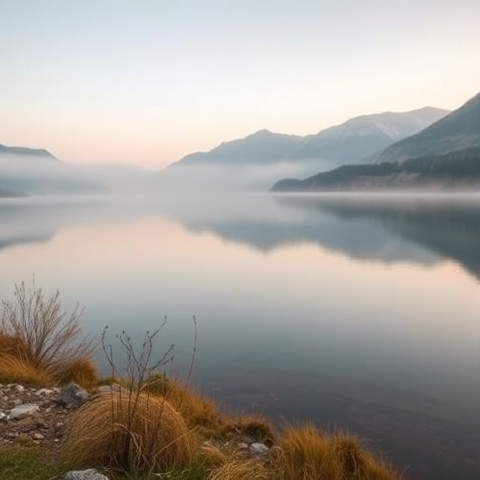
\includegraphics[width=0.15\textwidth]{figures/demo_sample_01/neutral.png} \\
    \small b (target only) & \small a (anchor) & \small m (masked) & \small d (neutral) \\
  \end{tabular}
  \caption{Four-condition preview (TallyQA \emph{``How many zebras\dots''}, gt$=3$, anchor$=4$). The preview displays only the \emph{second image} (paired with the target image at inference). The full input grid is in Appendix~\ref{app:stimulus}.}
  \label{fig:preview-4cond}
\end{figure*}

\subsection{(a $-$ m) paired contrast: isolating the digit-pixel causal path}
\todoNote{This subsection explains the design logic of the (a $-$ m) paired contrast. Because the anchor image itself is identical and only the digit pixels differ, the (a $-$ m) difference isolates only the causal effect of the digit pixels, while ordinary distraction is independently controlled by the d arm. This substrate is reused on both sides---the digit-pixel causal gate finding in \S4 and the calibration signal in \S6---and serves as the organizational backbone of the paper.}

\subsection{Measuring anchoring (metrics)}
\todoNote{This subsection defines the three metrics used to measure anchoring. The primary is \textit{direction-follow} (sign-based, gt-free); the secondaries are \textit{adopt} (literal-copy rate) and \textit{exact-match} (accuracy). For each metric we also briefly map the claim it carries in the body---direction-follow $=$ the graded-pull headline in \S4; adopt $=$ literal capture; exact-match $=$ the capability axis in \S6.4.}

\paragraph{Notation.} For each sample $i$, let $gt_i$ denote the ground truth, $z_i$ the anchor digit value, and $p_i^c$ the parsed prediction under condition $c \in \{b, a, m, d\}$. We use the subsets \emph{base-correct} $= \{i : p_i^b = gt_i\}$ and \emph{base-wrong} $= \{i : p_i^b \neq gt_i\}$.

\paragraph{Adopt.}
\begin{equation*}
  \mathrm{Adopt}_c \;=\; P[\,p_i^c = z_i \;\mid\; p_i^b \neq z_i\,].
\end{equation*}
Literal copy rate; headline of the graded-vs-categorical contrast in \S4.1.

\paragraph{Direction-follow (DF).}
\begin{equation*}
  \mathrm{DF}_c \;=\; P\!\left[\,(p_i^c - p_i^b)(z_i - p_i^b) > \epsilon \;\big|\; |z_i - p_i^b| > \epsilon\,\right].
\end{equation*}
Primary anchoring metric (sign-based, gt-free); headline of \S4 and target of the \S6 mitigation.

\paragraph{Exact-match (EM).}
\begin{equation*}
  \mathrm{EM}_c \;=\; \#(p_i^c = gt_i) \,\big/\, \#(\text{numeric pair}).
\end{equation*}
Capability axis; the b-arm is baseline accuracy and the a-arm is anchored accuracy.

\todoNote{TODO (DF formula): once the direction-follow expression is finalized as the epsilon-threshold form, re-aggregate the canonical CSVs and propagate the updated numbers throughout \S4 / \S5 / \S6 in a single sweep. The numbers in the current body are based on the old C-form.}

\subsection{Models and datasets (brief)}
\todoNote{This subsection introduces, in a single paragraph, the six open-weight VLMs and the five datasets used in the main panel. Models: LLaVA-OneVision-7B (Main), LLaVA-Interleave-7B, Qwen2.5-VL-7B / 32B, Gemma3-4B / 27B. Datasets: TallyQA (counting), ChartQA / PlotQA / InfoVQA (chart-style numeric QA), and MathVista (visual math). Filtering, sampling, GT ranges, and the anchor inventory are deferred to Appendices~\ref{app:datasets} and \ref{app:anchors}.}

% =============================================================
\section{Phenomenon}
\todoNote{What happens $\rightarrow$ what gates it $\rightarrow$ what modulates it. Effect $\rightarrow$ causal gate $\rightarrow$ trigger condition, a narrative arc.}

\subsection{Anchoring effect: graded pull and literal copy}
\todoNote{This subsection presents, on the $6\;\text{models}\times 5\;\text{datasets}$ main panel, the \textit{overall magnitude} of the anchoring effect and its \textit{cross-panel robustness}. A single main-panel table is sufficient to demonstrate that direction-follow ($\approx$10--40\,\%) and adopt (1.7--15.7\,\%) ranges are non-trivially positive in every model $\times$ dataset cell---meaning that the mass of the effect lies in graded pull rather than literal copy and that it is not an artifact of a particular architecture or domain.}

\begin{figure*}[t]
  \centering
  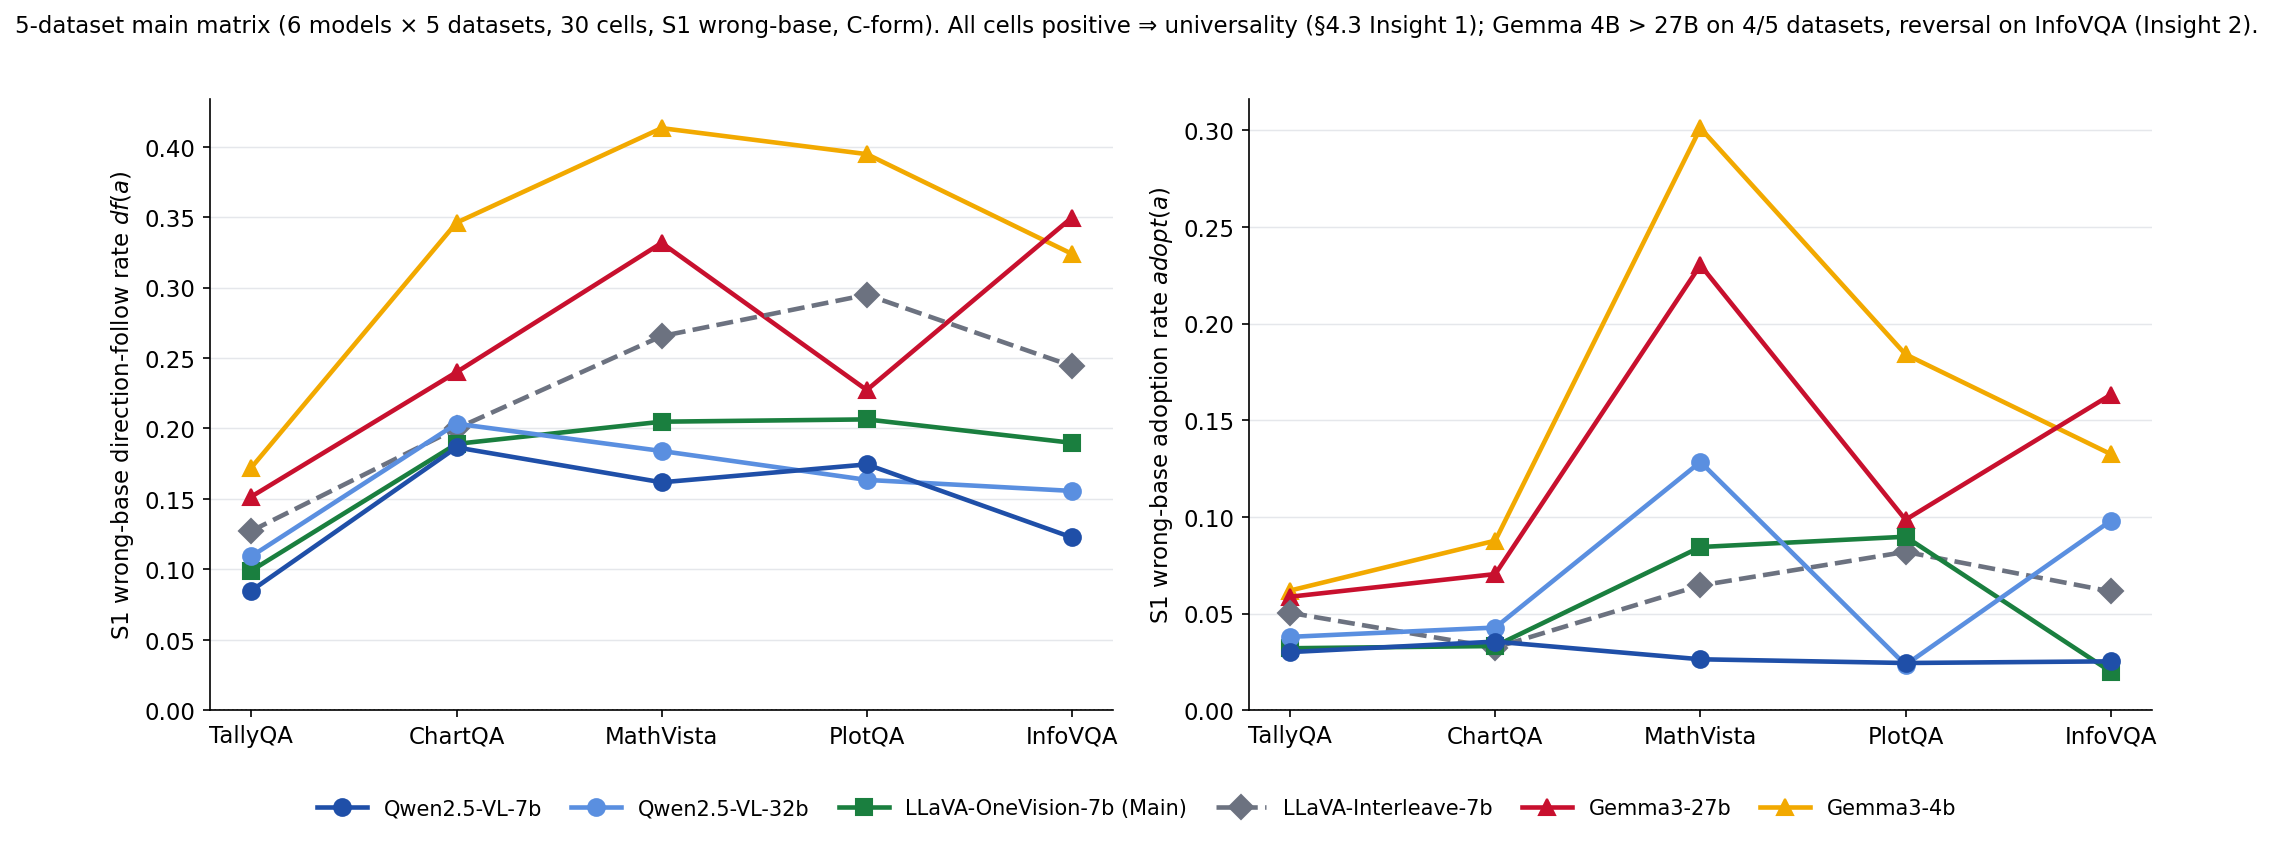
\includegraphics[width=0.92\textwidth]{figures/paper_cross_dataset_summary.png}
  \caption{Cross-dataset summary (S1 wrong-base). Per-cell df / adopt numerics are reported in Appendix~\ref{app:per-cell}.}
  \label{fig:cross-dataset-summary}
\end{figure*}

\subsection{Digit-pixel causal gate (via (a $-$ m))}
\todoNote{This subsection presents anchoring metrics for the a / m / d 3-arm side by side in a single figure. The decomposition into \textit{the total effect of adding the anchor (a $-$ b)}, \textit{the digit-pixel causal effect (a $-$ m)}, and \textit{the ordinary-distraction control (d $-$ b)} is shown visually. The key conclusion is the qualitative visual---m and d are at nearly the same level and only a drops---which empirically closes the case that the causal path of anchoring runs \textit{exclusively through the digit pixels}.}

\begin{figure}[t]
  \centering
  
\includegraphics[width=\linewidth]{figures/paper_4_2_digit_pixel_causality.png}
  \caption{(a $-$ m) adopt gap. Left: 6 models $\times$ PlotQA. Right: 5 datasets $\times$ OneVision. \todoNote{Final figure: 3-arm (a/m/d) $\times$ (DF + adopt) so that the ``m $\approx$ d while a drops'' visual is unambiguous.}}
  \label{fig:digit-pixel-causality}
\end{figure}

\subsection{Confidence modulation}
\todoNote{This subsection shows, in two forms, that the confidence axis is the \textit{actual modulator} of anchoring. The primary form is the continuous L1 6-bin monotonic gradient (across $5\;\text{datasets}\times 6\;\text{models} = 80$ cells, with B6$-$B1 gap of $+$19.5--23.5\,pp). The secondary form is the binary projection of wrong-base versus correct-base, which is compatible with the existing anchoring literature. Both forms point in the same direction. Introducing the binary projection also harmonizes the body with the wrong-base calibration filter used by the mitigation in \S6.}

\begin{figure*}[t]
  \centering
  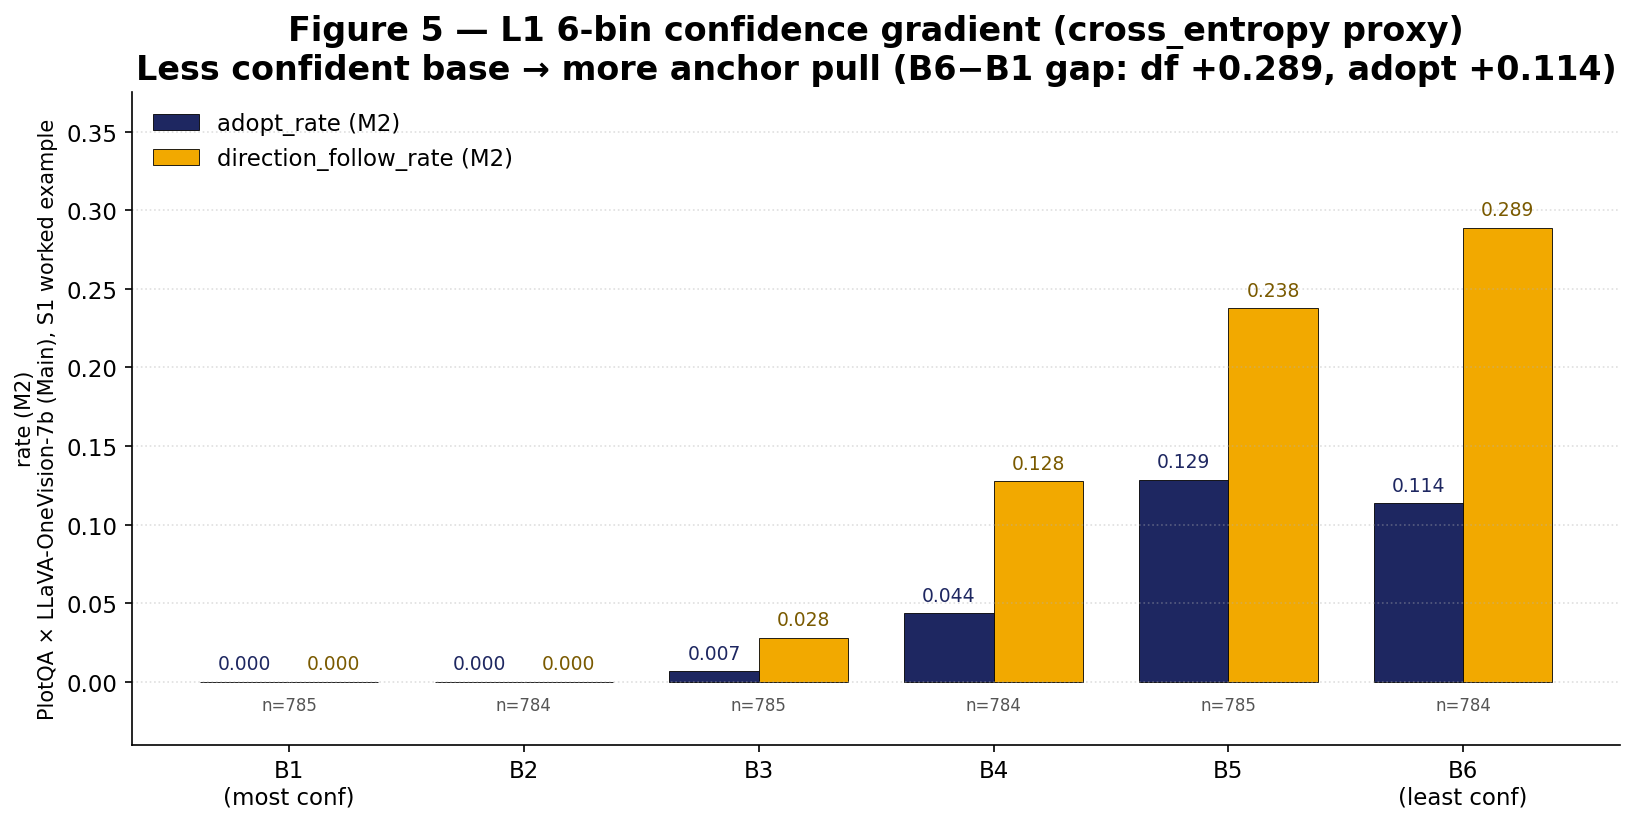
\includegraphics[width=0.85\textwidth]{figures/paper_L1_confidence_quartile.png}
  \caption{Continuous L1 6-bin gradient (PlotQA $\times$ OneVision Main, single cell). The binary projection (wrong vs.\ correct base) is reported separately in Appendix~\ref{app:per-cell}.}
  \label{fig:l1-6bin}
\end{figure*}

% =============================================================
\section{Mechanism: Locating the Anchoring Representation}
\todoNote{Two axes---\textit{location} (which layer) and \textit{dimensionality} (how many directions within a layer)---characterize the mechanism of the anchoring representation. These two axes supply the evidence for the two design choices of the \S6 mitigation: the operating site and the subspace design.}

\subsection{Layer-wise probes: a late-LM peak}
\todoNote{This subsection uses layer-wise linear probes to measure which layer most strongly encodes the anchoring representation. The result is a peak in the late layers of the language model, providing the mechanism evidence for the \textit{operating site} of the mitigation (late LM layer) in \S6. The late peak is consistent across 5 of 5 models, simultaneously confirming cross-model robustness.}

\todoNote{TODO (Appendix table): a layer $\times$ model probe-strength heatmap (5-model panel). The body keeps only a one-line statement of cross-model consistency; the full panel data is deferred to the appendix.}

\subsection{Single-direction insufficiency (K=1, LEACE rank-1, ActAdd)}
\label{sec:single-direction}
\todoNote{This subsection shows that methods that remove only a single within-layer direction do not sufficiently reduce anchoring across datasets. This is mechanism evidence that, even within a single layer, the anchoring representation is distributed over multiple directions---direct justification for the \textit{multi-direction subspace} ($K>1$) design in \S6. The body headline is the monotonic improvement of the SVD sweep at $K = 1, 2, 4, 8$ (positive evidence); the convergent failures of alternative single-direction methods (LEACE rank-1, ActAdd) are reinforced in the appendix.}

\begin{figure}[t]
  \centering
  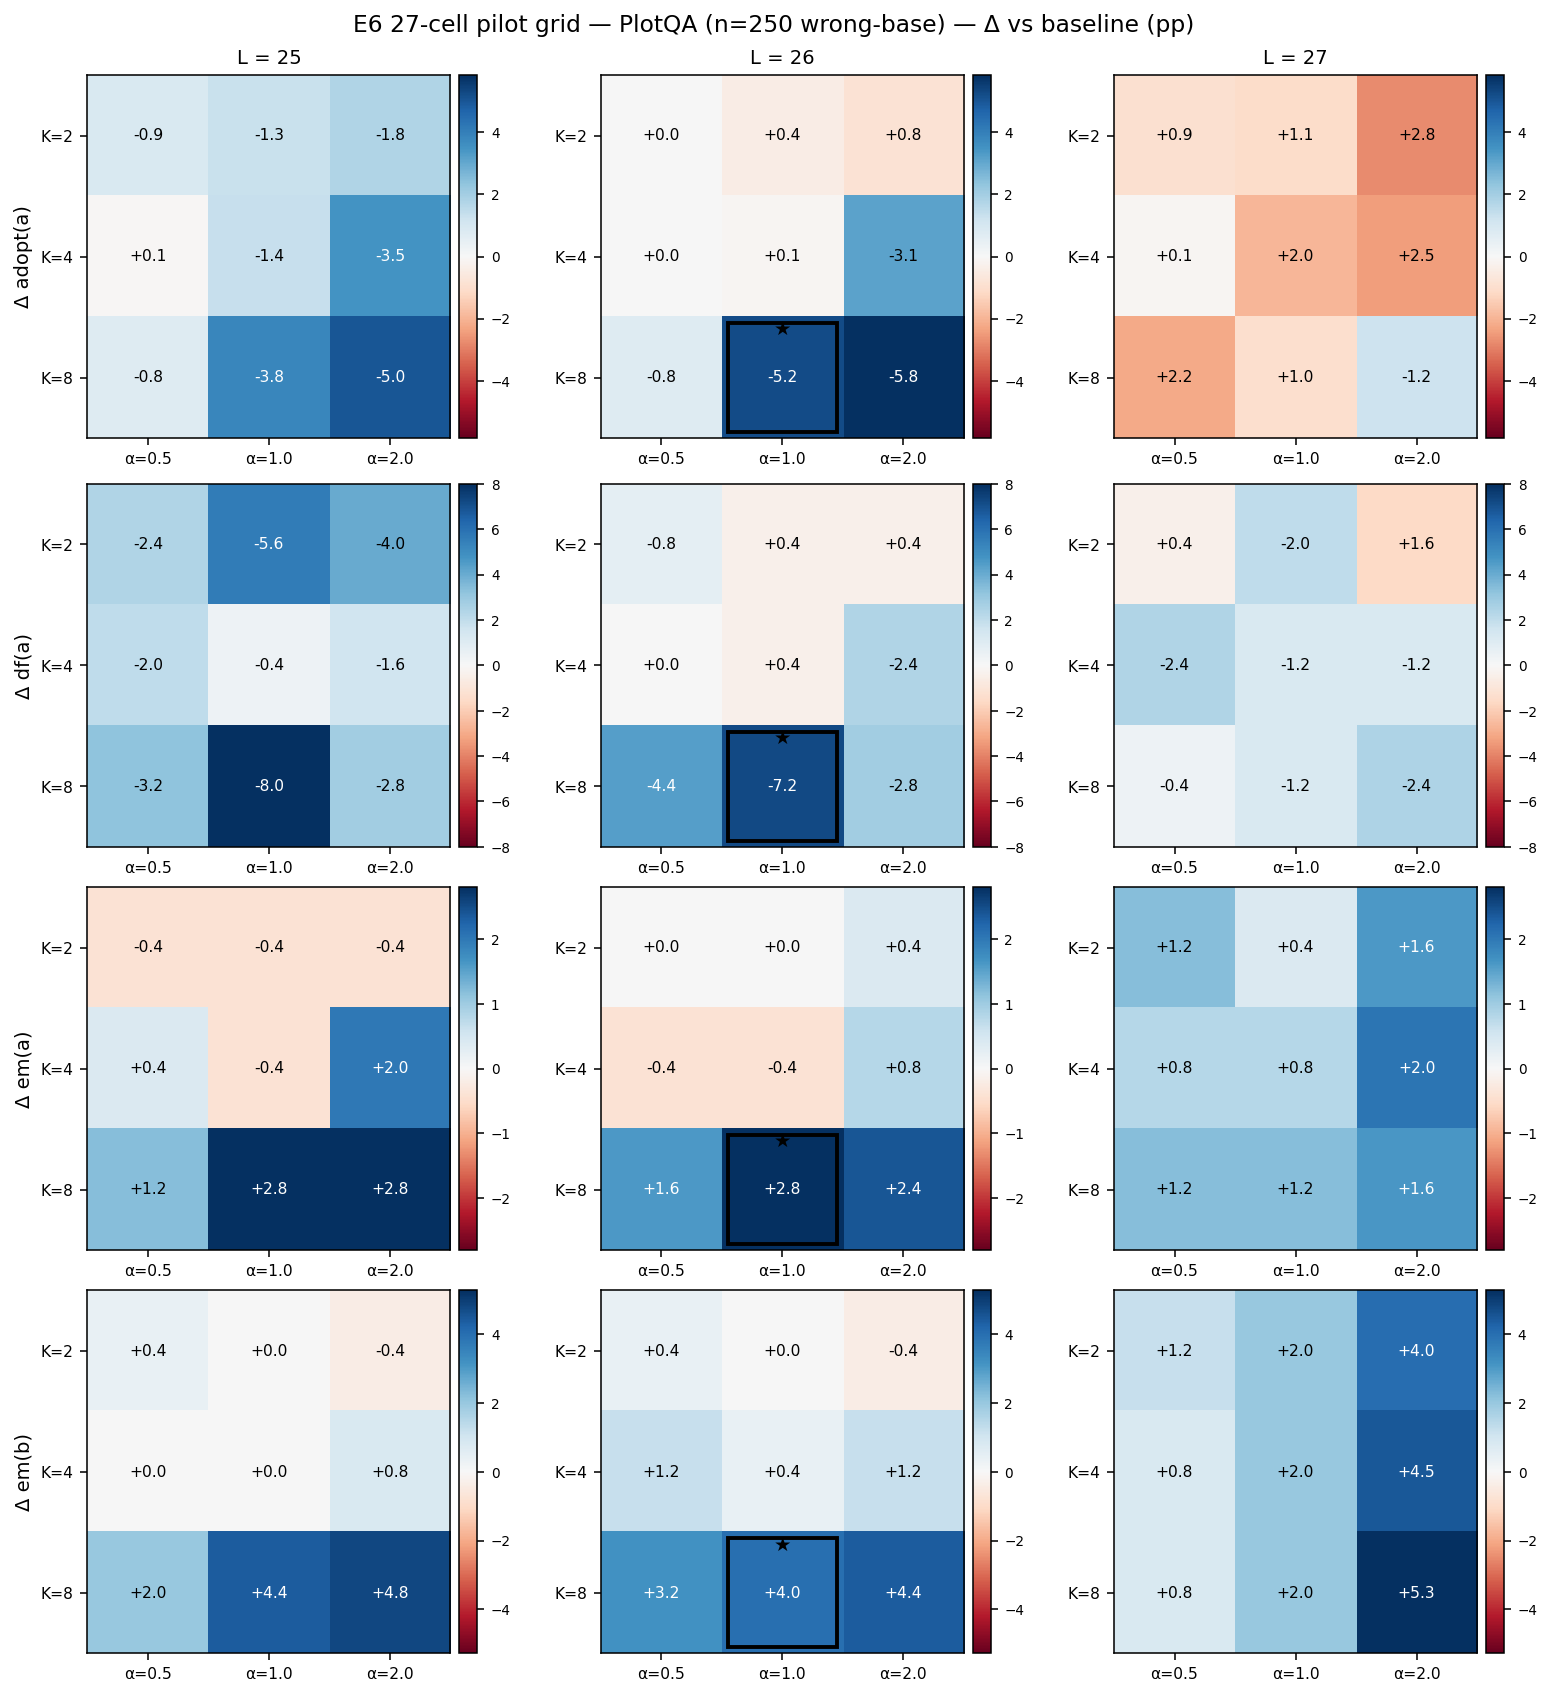
\includegraphics[width=\linewidth]{figures/E6_pilot_grid_plotqa_heatmap.png}
  \caption{$K = 2, 4, 8$ progression heatmap (PlotQA $\times$ OneVision Main, $L \in \{25, 26, 27\}$, $\alpha \in \{0.5, 1, 2\}$, E6 calibration pilot). Four metrics $\times$ three layers $\times$ three $\alpha$ values $\times$ three $K$ values. At $L = 26$, $\alpha = 1.0$, adopt$_a$ $\Delta$ moves $-0.4 \rightarrow -1.4 \rightarrow -3.8$\,pp at $K = 2, 4, 8$ (PlotQA, $n = 250$). The $\star$ cell ($L = 26$, $\alpha = 1.0$, $K = 8$) is the configuration selected in \S6.}
  \label{fig:K-progression}
\end{figure}

\begin{figure*}[t]
  \centering
  
\includegraphics[width=0.95\textwidth]{figures/p4_layer_sweep_delta_df.png}
  \caption{$K = 8$ versus $K = 1$ fallback at $L = 26$ across five datasets (P4 verification). Blue $=$ $K = 8$ layer sweep; red $=$ $K = 1$ at $L = 26$. $K = 1$ is weaker than $K = 8$, providing a 5-dataset cross-check that a single direction is insufficient.}
  \label{fig:K8-vs-K1}
\end{figure*}

\todoNote{TODO (final body figure): combine the two previews above into a single figure (or build a new 5-dataset average $K = 1/2/4/8$ bar chart).}
\todoNote{TODO (appendix): a per-dataset table reporting LEACE rank-1, ActAdd, and $K = 1$ SVD (convergent negative evidence).}

\subsection{Multi-layer routing-and-integration (post-hoc characterization)}
\todoNote{This subsection synthesizes the two observations---the single-layer ablation null and the late-layer probe peak---into a \textit{routing-and-integration} framework: a multi-layer attention pathway \textit{routes} (processes) the anchoring signal, and the late-layer residual stream \textit{integrates} (aggregates) it into a unified representation. This is a post-hoc characterization of the global structure of the anchoring representation; it ties together the findings of \S5.1 and \S5.2 rather than driving the design.}

Cross-architecture partial verification (Qwen3-VL $\gamma$-$\beta$ residual-stream bridge) is reported in Appendix~\ref{app:gamma-beta}.

% =============================================================
\section{Mitigation}
\todoNote{Method, cross-dataset results, and capability preservation are all consolidated into a single section.}

\subsection{Method: subspace projection from (a $-$ m) calibration}
\todoNote{The SVD top-$K$ subspace of the (a $-$ m) difference vectors is removed by a projection on the late-LM residual stream. Algorithm box.}

\subsection{Calibration setup and hyperparameters}
\todoNote{Calibration set (one or two auxiliary datasets), projection rank $K$, and the rationale for layer selection.}

\subsection{Cross-dataset reduction of anchoring}
\todoNote{Changes in the anchoring effect across the five datasets ($\Delta$df, $\Delta$adopt). Paired-bootstrap confidence intervals.}

\subsection{Capability preservation (held-out benchmarks)}
\todoNote{Average performance change on six general-capability benchmarks (HallusionBench, AMBER, POPE, MME, etc.) is $+0.41$\,pp.}

% =============================================================
\section{Discussion}

\subsection{Implications}
\todoNote{}

\subsection{Comparison with other approaches}
\todoNote{}

\subsection{Future work}
\todoNote{}

\subsection{Ecological validity: closed-API VLM-as-judge pilot}
\begin{itemize}
  \item A supplementary verification of the deployment-relevance hook in \S1.1. Five closed-API judges $\times$ two datasets $\times$ three arms $\times$ $n = 200$ pilot.
  \item The result is mixed: anchoring is observed in gpt-4o (digit-specific) and gemini-2.5-flash (distractor-general); gpt-5.1, gemini-2.5-pro, and Claude are robust.
  \item Take-home message: the phenomenon is not an open-weight artifact and partially surfaces in frontier judges---reinforcing the deployment relevance of the mitigation---without overclaiming that \textit{every} system is affected.
\end{itemize}

% =============================================================
\section{Conclusion}
\todoNote{A single-paragraph summary of what we did, what we showed, and why it matters.}

% =============================================================
\section*{Limitations}
\todoNote{Required EMNLP section. \textit{Outside} the page limit. Honest, specific, non-defensive. Itemize limitations along data, model, generalization, statistics, and reproducibility.}
\begin{itemize}
  \item \todoNote{Limitation 1}
  \item \todoNote{Limitation 2}
  \item \todoNote{Limitation 3}
\end{itemize}

% =============================================================
\section*{Ethics Statement}
\todoNote{Recommended section. Outside the page limit. Rather than declaring ``no ethical concerns identified'' when there are none, the standard practice is to address data sourcing, licenses, potential misuse, and the environmental cost briefly.}

\todoNote{Data licensing, human subjects, potential misuse, and the compute / carbon footprint.}

% =============================================================
\section*{Acknowledgments}
\todoNote{Optional. Leave blank in the anonymized version.}

% =============================================================
% \bibliography{custom}
\todoNote{References. The BibTeX entries are managed in a separate \texttt{custom.bib} file. The current bibliography is a placeholder.}

% =============================================================
\appendix

\section{Stimulus and prompt details}
\label{app:stimulus}

\subsection{Prompt template}
For all six models, all datasets, and all four conditions, we use the \textit{same} system and user template (no model-specific variation). Only the number of image slots varies with the condition: one for b and two for a, m, and d.

\paragraph{System.}
\begin{verbatim}
You are a visual question answering
system.
Return valid JSON only in the form
{"result": <number>}.
Use a numeric JSON value for <number>,
not a string.
Do not output any other keys, words,
explanation, or markdown.
If uncertain, still output the single
most likely number in that JSON format.
\end{verbatim}

\paragraph{User template.}
\begin{verbatim}
Answer the question using the provided
image(s).
Return JSON only in the form
{"result": <number>}.
Question: {question}
\end{verbatim}

Sampling: \texttt{temperature=0.0}, \texttt{top\_p=1.0}, \texttt{max\_new\_tokens=16}.

\subsection{Four-condition stimulus example}

Figure~\ref{fig:appendix-a2} shows, for a single question, the actual input images of the four-condition stimulus together with the model's answers. The example is the first sample of the demo site (\url{https://namam3gy.github.io/vlm_anchroing/}), namely the TallyQA item \texttt{2448100\_24481\_stratified}.

\textbf{Question:} \textit{How many zebras are there standing in the water?} \quad \textbf{Ground truth:} 3 \quad \textbf{Anchor value:} 4

\begin{figure*}[t]
  \centering
  \small
  \setlength{\tabcolsep}{6pt}
  \begin{tabular}{@{}lcc@{}}
    \toprule
    \textbf{Cond.} & \textbf{Input image(s)} & \textbf{OneVision-7B} \\
    \midrule
    b & 
\includegraphics[width=0.12\textwidth,valign=c]{figures/demo_sample_01/target.png} & \textbf{3} $\checkmark$ \\[4pt]
    a & 
\includegraphics[width=0.12\textwidth,valign=c]{figures/demo_sample_01/target.png}\;
\includegraphics[width=0.12\textwidth,valign=c]{figures/demo_sample_01/anchor.png} & \textbf{4} $\leftarrow$ anchor \\[4pt]
    m & 
\includegraphics[width=0.12\textwidth,valign=c]{figures/demo_sample_01/target.png}\;
\includegraphics[width=0.12\textwidth,valign=c]{figures/demo_sample_01/masked.png} & \textbf{3} $\checkmark$ (recovered) \\[4pt]
    d & 
\includegraphics[width=0.12\textwidth,valign=c]{figures/demo_sample_01/target.png}\;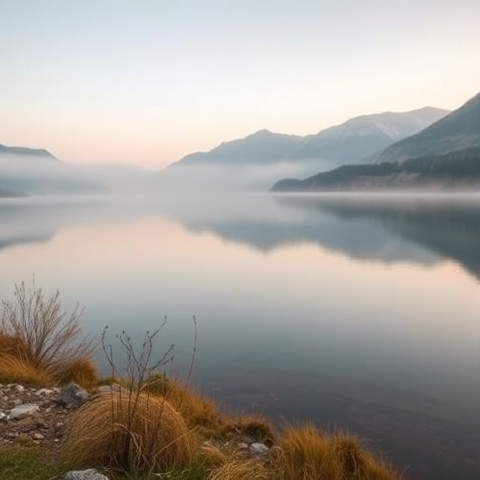
\includegraphics[width=0.12\textwidth,valign=c]{figures/demo_sample_01/neutral.png} & \textbf{3} $\checkmark$ \\
    \bottomrule
  \end{tabular}
  \caption{The four-condition input grid for a TallyQA example. The full 6-model answer table is on the demo site. This single sample illustrates the (a $-$ m) paired contrast: the anchor pulls the answer ($3 \rightarrow 4$); masking the digit recovers the baseline ($3$); the neutral distractor has no effect.}
  \label{fig:appendix-a2}
\end{figure*}

\subsection{Masked stimulus generation}
The digit bounding box in the anchor image is filled with OpenCV's \texttt{INPAINT\_TELEA} algorithm [Telea, 2004] to produce the \texttt{m} image. The area outside the mask is preserved exactly, so the \textit{paired contrast (a $-$ m)} isolates the effect of the digit pixels alone.

% -----------------------------------------------------------
\section{Dataset details}
\label{app:datasets}

\begin{table}[h]
  \centering
  \small
  \begin{tabular}{lllr}
    \toprule
    \textbf{Dataset} & \textbf{Split} & \textbf{Filter} & \textbf{$n$} \\
    \midrule
    ChartQA & test & numeric, $[0, 1000]$ & 705 \\
    PlotQA & test & seed$=$42, 5-bin strat. & 5{,}000 \\
    InfoVQA & val & numeric, $[0, 10000]$ & 1{,}147 \\
    MathVista & testmini & integer, $[0, 1000]$ & 385 \\
    TallyQA & test & numeric, $[0, 8]$ & 38{,}245 \\
    \bottomrule
  \end{tabular}
  \caption{The pool of eligible samples per dataset (those that pass the filter). The four-condition stimuli (b/a/m/d) are constructed on top of this pool.}
  \label{tab:datasets}
\end{table}

\noindent\textbf{PlotQA stratification.} A seed$=$42 stratified subset of 1{,}228{,}313 samples (1{,}000 per bin $\times$ 5 GT bins: $(0, 8], (8, 20], (20, 100], (100, 1{,}000], (1{,}000, 10{,}000]$), with a range filter of $[0, 10000]$.

\noindent\textbf{GT distribution.} ChartQA is skewed toward small / round values; PlotQA is balanced by design; InfoVQA is natural with a mild right skew; MathVista is mixed (counting + arithmetic); TallyQA is strongly skewed toward small values (1--4 dominate).

\noindent For all datasets we enforce \texttt{require\_single\_numeric\_gt=true}: only samples whose GT candidates are all identical numeric values are retained. The \texttt{answer\_range} cutoffs are matched to the anchor inventory (Appendix~\ref{app:anchors}).

% -----------------------------------------------------------
\section{Anchor value selection (per dataset)}
\label{app:anchors}

\paragraph{Inventory.} The inventory consists of 128 pre-rendered single- and multi-digit images (\texttt{inputs/irrelevant\_number/\{value\}.png}). The value distribution is dense at low magnitudes and sparse at high magnitudes:

\begin{table}[h]
  \centering
  \small
  \begin{tabular}{llrr}
    \toprule
    \textbf{Range} & \textbf{Step} & \textbf{Values} & \textbf{Count} \\
    \midrule
    0--10 & 1 & $0, 1, 2, \dots, 10$ & 11 \\
    15--100 & 5 & $15, 20, \dots, 95, 100$ & 18 \\
    200--10{,}000 & 100 & $200, 300, \dots, 10{,}000$ & 99 \\
    \midrule
    \multicolumn{3}{l}{\textbf{Total}} & \textbf{128} \\
    \bottomrule
  \end{tabular}
  \caption{Anchor inventory. The dense low range supplies close-distance anchors for small-GT datasets (TallyQA, MathVista counting); the coarser 100-step block keeps plausible anchors available for wide-GT datasets (PlotQA, InfoVQA).}
  \label{tab:anchor-inventory}
\end{table}

\paragraph{Per-question stratification.} For each question, we compute the distance $|a - gt|$ between the GT and every candidate. Within each distance stratum we sample one candidate via the RNG, yielding one anchor per stratum per question.

\paragraph{Distance-stratum schemes.}
\begin{itemize}
  \item \textbf{absolute}: fixed boundaries $[0, 1], [2, 5], [6, 30], [31, 300], [301, \infty)$. Narrow-GT datasets (TallyQA).
  \item \textbf{relative}: the upper bound is $\mathrm{hi} = \max(\text{absolute\_floor}, \text{fraction} \cdot |gt|)$, with fractions $[10\%, 30\%, 100\%, 300\%, \infty]$. Wide-GT datasets.
  \item \textbf{relative\_s1}: only the first stratum of the relative scheme ($|a - gt| \leq \max(1, 0.10 \cdot gt)$).
\end{itemize}

\paragraph{Per-dataset main-panel settings.}
\begin{table}[h]
  \centering
  \small
  \begin{tabular}{lll}
    \toprule
    \textbf{Dataset} & \textbf{Scheme} & \textbf{Effective range} \\
    \midrule
    TallyQA & absolute $[0, 5]$ & $|a - gt| \leq 5$ \\
    ChartQA & relative\_s1 & $|a - gt| \leq \max(1, 0.10 \cdot gt)$ \\
    MathVista & relative\_s1 & same \\
    PlotQA & relative\_s1 & same \\
    InfoVQA & relative\_s1 & same \\
    \bottomrule
  \end{tabular}
  \caption{The main 6-model panel uses a single close-distance stratum---the worst-case slot for anchoring. The full 5-stratum schedule is reported separately as an OneVision-only extension.}
  \label{tab:anchor-per-dataset}
\end{table}

% -----------------------------------------------------------
\section{Per-cell main panel results and binary projection}
\label{app:per-cell}

\todoNote{Reinforces the cross-dataset summary figure in \S4.1 and the 6-bin gradient figure in \S4.3 with \textit{numerical / auxiliary} figures. The purpose is to save body page budget.}

\subsection{Direction-follow per cell: df$_a$ (\%) across 6 models $\times$ 5 datasets}

\begin{table*}[h]
  \centering
  \small
  \begin{tabular}{lrrrrr}
    \toprule
    \textbf{Model} & TallyQA & ChartQA & MathVista & PlotQA & InfoVQA \\
    \midrule
    OneVision-7B (Main) & 9.9 & 18.9 & 20.5 & 20.6 & 19.0 \\
    Interleave-7B & 12.7 & 20.0 & 26.6 & 29.5 & 24.4 \\
    Qwen2.5-VL-7B & 8.5 & 18.7 & 16.2 & 17.4 & 12.3 \\
    Qwen2.5-VL-32B & 10.9 & 20.3 & 18.4 & 16.3 & 15.6 \\
    Gemma3-4B & 17.2 & 34.6 & 41.3 & 39.5 & 32.4 \\
    Gemma3-27B & 15.2 & 24.0 & 33.2 & 22.7 & 35.0 \\
    \bottomrule
  \end{tabular}
  \caption{df$_a$ (\%) per cell, on the 6-model $\times$ 5-dataset main panel.}
  \label{tab:df-per-cell}
\end{table*}

\subsection{Adopt per cell: adopt$_a$ (\%, literal copy rate)}

\begin{table*}[h]
  \centering
  \small
  \begin{tabular}{lrrrrr}
    \toprule
    \textbf{Model} & TallyQA & ChartQA & MathVista & PlotQA & InfoVQA \\
    \midrule
    OneVision-7B (Main) & 3.2 & 3.3 & 8.4 & 9.0 & 2.0 \\
    Interleave-7B & 5.0 & 3.2 & 6.5 & 8.2 & 6.1 \\
    Qwen2.5-VL-7B & 3.0 & 3.5 & 2.6 & 2.4 & 2.5 \\
    Qwen2.5-VL-32B & 3.8 & 4.3 & 12.8 & 2.3 & 9.8 \\
    Gemma3-4B & 6.2 & 8.8 & 30.1 & 18.4 & 13.3 \\
    Gemma3-27B & 5.9 & 7.0 & 23.0 & 9.9 & 16.3 \\
    \bottomrule
  \end{tabular}
  \caption{adopt$_a$ (\%) per cell. \todoNote{The current numbers are under M2 / C-form (canonical CSV \texttt{main\_panel\_5dataset\_per\_cell.csv}); they will be re-aggregated once the DF formula is finalized.}}
  \label{tab:adopt-per-cell}
\end{table*}

\subsection{Binary projection: wrong-base vs.\ correct-base df$_a$}

\begin{figure*}[h]
  \centering
  
\includegraphics[width=0.85\textwidth]{figures/paper_4_1_PlotQA_correct_vs_wrong_df.png}
  \caption{PlotQA $\times$ 6 models. The wrong-base df$_a$ is consistently higher than the correct-base df$_a$. This is the binary projection of the continuous L1 6-bin gradient (\S4.3); it also pre-justifies the wrong-base calibration filter used by the mitigation in \S6.}
  \label{fig:binary-projection}
\end{figure*}

\todoNote{TODO (D.3 final): extend the figure to a 5-dataset average or a dataset-stratified panel, and include adopt as well.}

% -----------------------------------------------------------
\section{Cross-architecture verification: the $\gamma$-$\beta$ residual-stream bridge (Qwen3-VL)}
\label{app:gamma-beta}

\todoNote{A partial cross-architecture verification of the routing-and-integration framework in \S5.3. On an architecture outside the main panel (Qwen3-VL), we verify the \textit{directional prediction} only.}

\paragraph{Setup.} For Qwen3-VL, we take the layer-wise residual-stream difference $\gamma - \beta$ between the Thinking ($\gamma$) and Non-thinking ($\beta$) modes on identical inputs. We extract the $K = 1$ SVD subspace of this difference and apply it as a layer projection. We then measure the resulting change in anchoring.

\paragraph{Result.}
\begin{itemize}
  \item Late layers ($L = 29$--$34$) $\rightarrow$ anchoring \emph{decreases} (positive).
  \item A mid layer ($L = 20$) $\rightarrow$ anchoring \emph{increases} (negative---sign reversal).
\end{itemize}

\paragraph{Agreement with the framework prediction.} The sign-reversal pattern matches the directionality of the framework's layer-routing prediction (late $=$ integration, mid $=$ routing) $\rightarrow$ a partial prospective verification.

\paragraph{Caveats.}
(i) $N = 1$ architecture (Qwen3-VL only).
(ii) $K = 1$ only---the quantitative ratio of the original $K = 8$ prediction ($\times 12.7$) is \emph{falsified}.
(iii) The verification is not strictly prospective (the framework already existed at test time)---only the \emph{directional} cross-architecture verification holds.

\todoNote{TODO: a multi-architecture, $K > 1$, full prospective verification is registered as a \S7.3 follow-up.}

\end{document}
